\section{Introduction}
%Each section needs a subsection for the small points on top to show up
\subsection{Dummy}

\begin{frame}{Electronic properties of quasicrystals}

Under the supervision of Anuradha Jagannathan

In collaboration with: Michel Duneau, Pavel Kalugin, Rémi Mosseri, Frédéric Piéchon.

\begin{itemize}
	\only<1>{
	\item {\ss{Fractal dimensions of wave functions and local spectral measures on the Fibonacci chain}\\\emph{Macé, Jagannathan, Piéchon, PRB 93 (20), 2016}}
	}

	\only<2>{
	\item \textbf{\ss Fractal dimensions of wave functions and local spectral measures on the Fibonacci chain}\\
	\textbf{\textit{\ss Macé, Jagannathan, Piéchon, PRB 93 (20), 2016}}
	}	
	
	\item {\ss{Quantum simulation of a 2D quasicrystal with cold atoms}\\
	\emph{Macé, Jagannathan, Duneau, Crystals 6 (10), 124}}

	\only<1>{
	\item {\ss{Critical eigenstates and their properties in one-and two-dimensional quasicrystals}\\
	\emph{Macé, Jagannathan, Kalugin, Mosseri, Piéchon, PRB 96 (4), 2017}}
	}
	
	\only<2>{
	\item \textbf{\ss{Critical eigenstates and their properties in one-and two-dimensional quasicrystals}}\\
	\textbf{\textit{\ss Macé, Jagannathan, Kalugin, Mosseri, Piéchon, PRB 96 (4), 2017}}
	}
	
	\item {\ss{Gap structure of 1D cut and project Hamiltonians}\\
	\emph{Macé, Jagannathan, Piéchon, J. Phys.: Conference Series 809 (1), 012023	}}
\end{itemize}

\end{frame}

\begin{frame}{Electronic properties of quasicrystals}
\(
	\<{6cm}
		\centering
		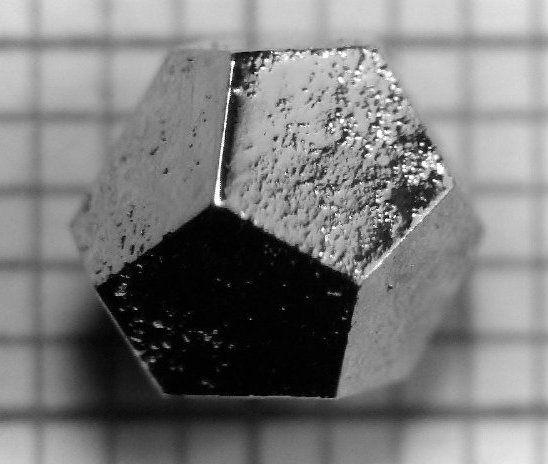
\includegraphics[scale=0.28]{img/1_intro/homgzn.png}
		
		\ss{3D HoMgZn quasicrystalline sample} \ss{(\url{doi:10.1038/nmat1244})}
	\>
	\<{6cm}
		\centering
		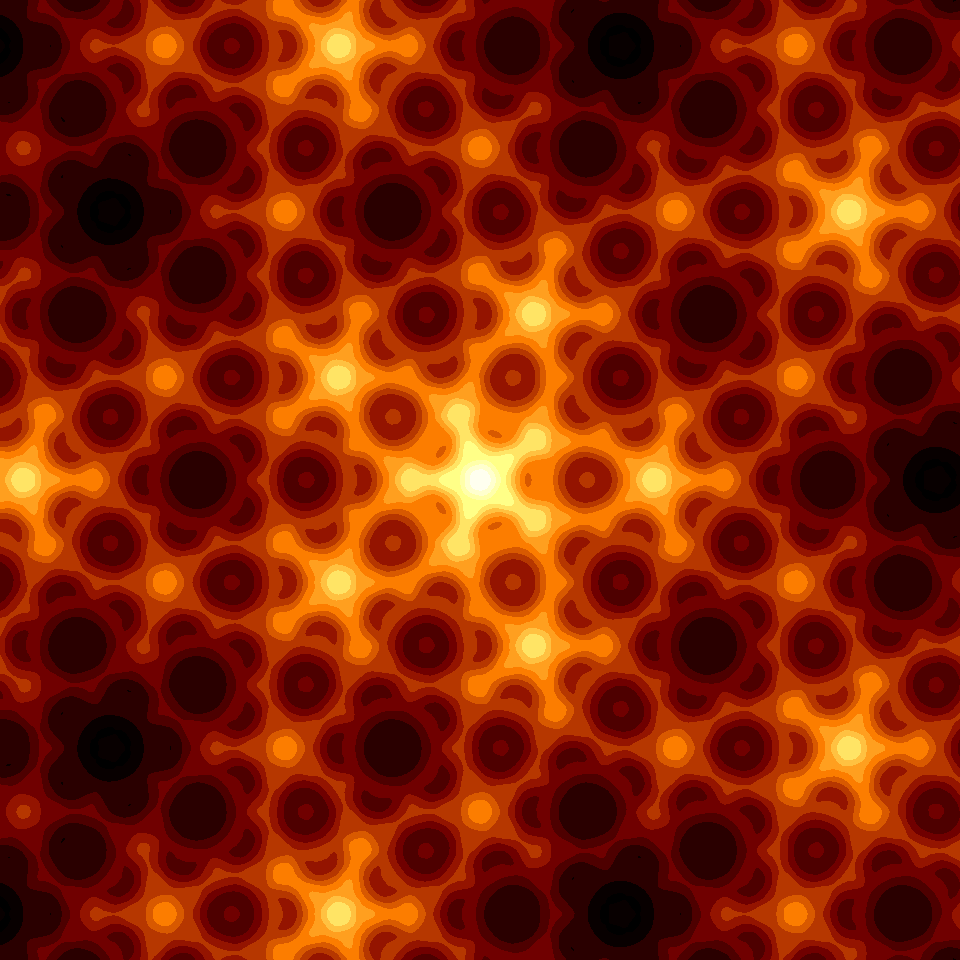
\includegraphics[scale=0.374]{img/1_intro/afmhot}
		
		\ss{Groundstate electron density} \ss{(simple tight-binding model on a 2D tiling)}
	\>
\)
Quasicrystals: not periodic yet ordered structures (discovery: 1982).

Here: single electron properties of tight-binding quasiperiodic models.
\end{frame}

\begin{frame}{A quasiperiodic puzzle [Bédaride \etal{} 12]}

\centering
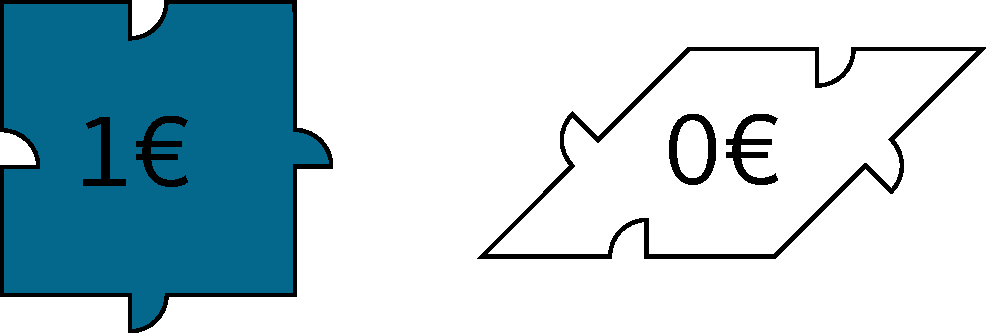
\includegraphics[width=.4\textwidth]{img/1_intro/tiles_euro.pdf}

Pay the squares, get the rhombuses for free!

\(
\<{6cm}
\centering
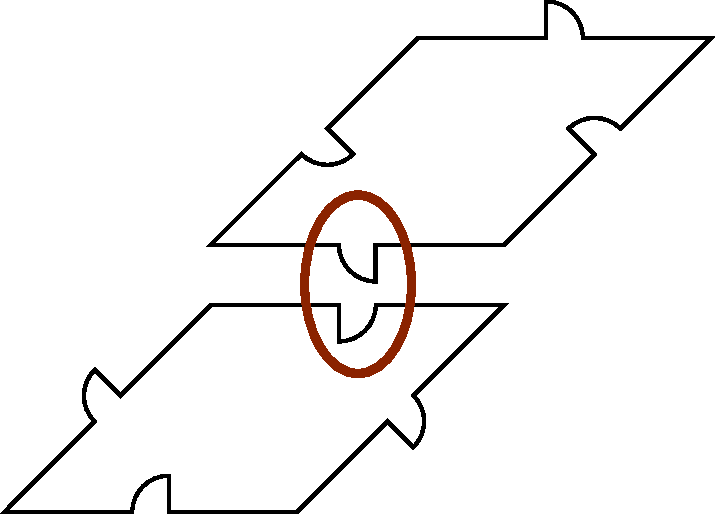
\includegraphics[width=.8\textwidth]{img/1_intro/forbidden.pdf}

Forbidden configuration.
\>

\<{6cm}
\centering
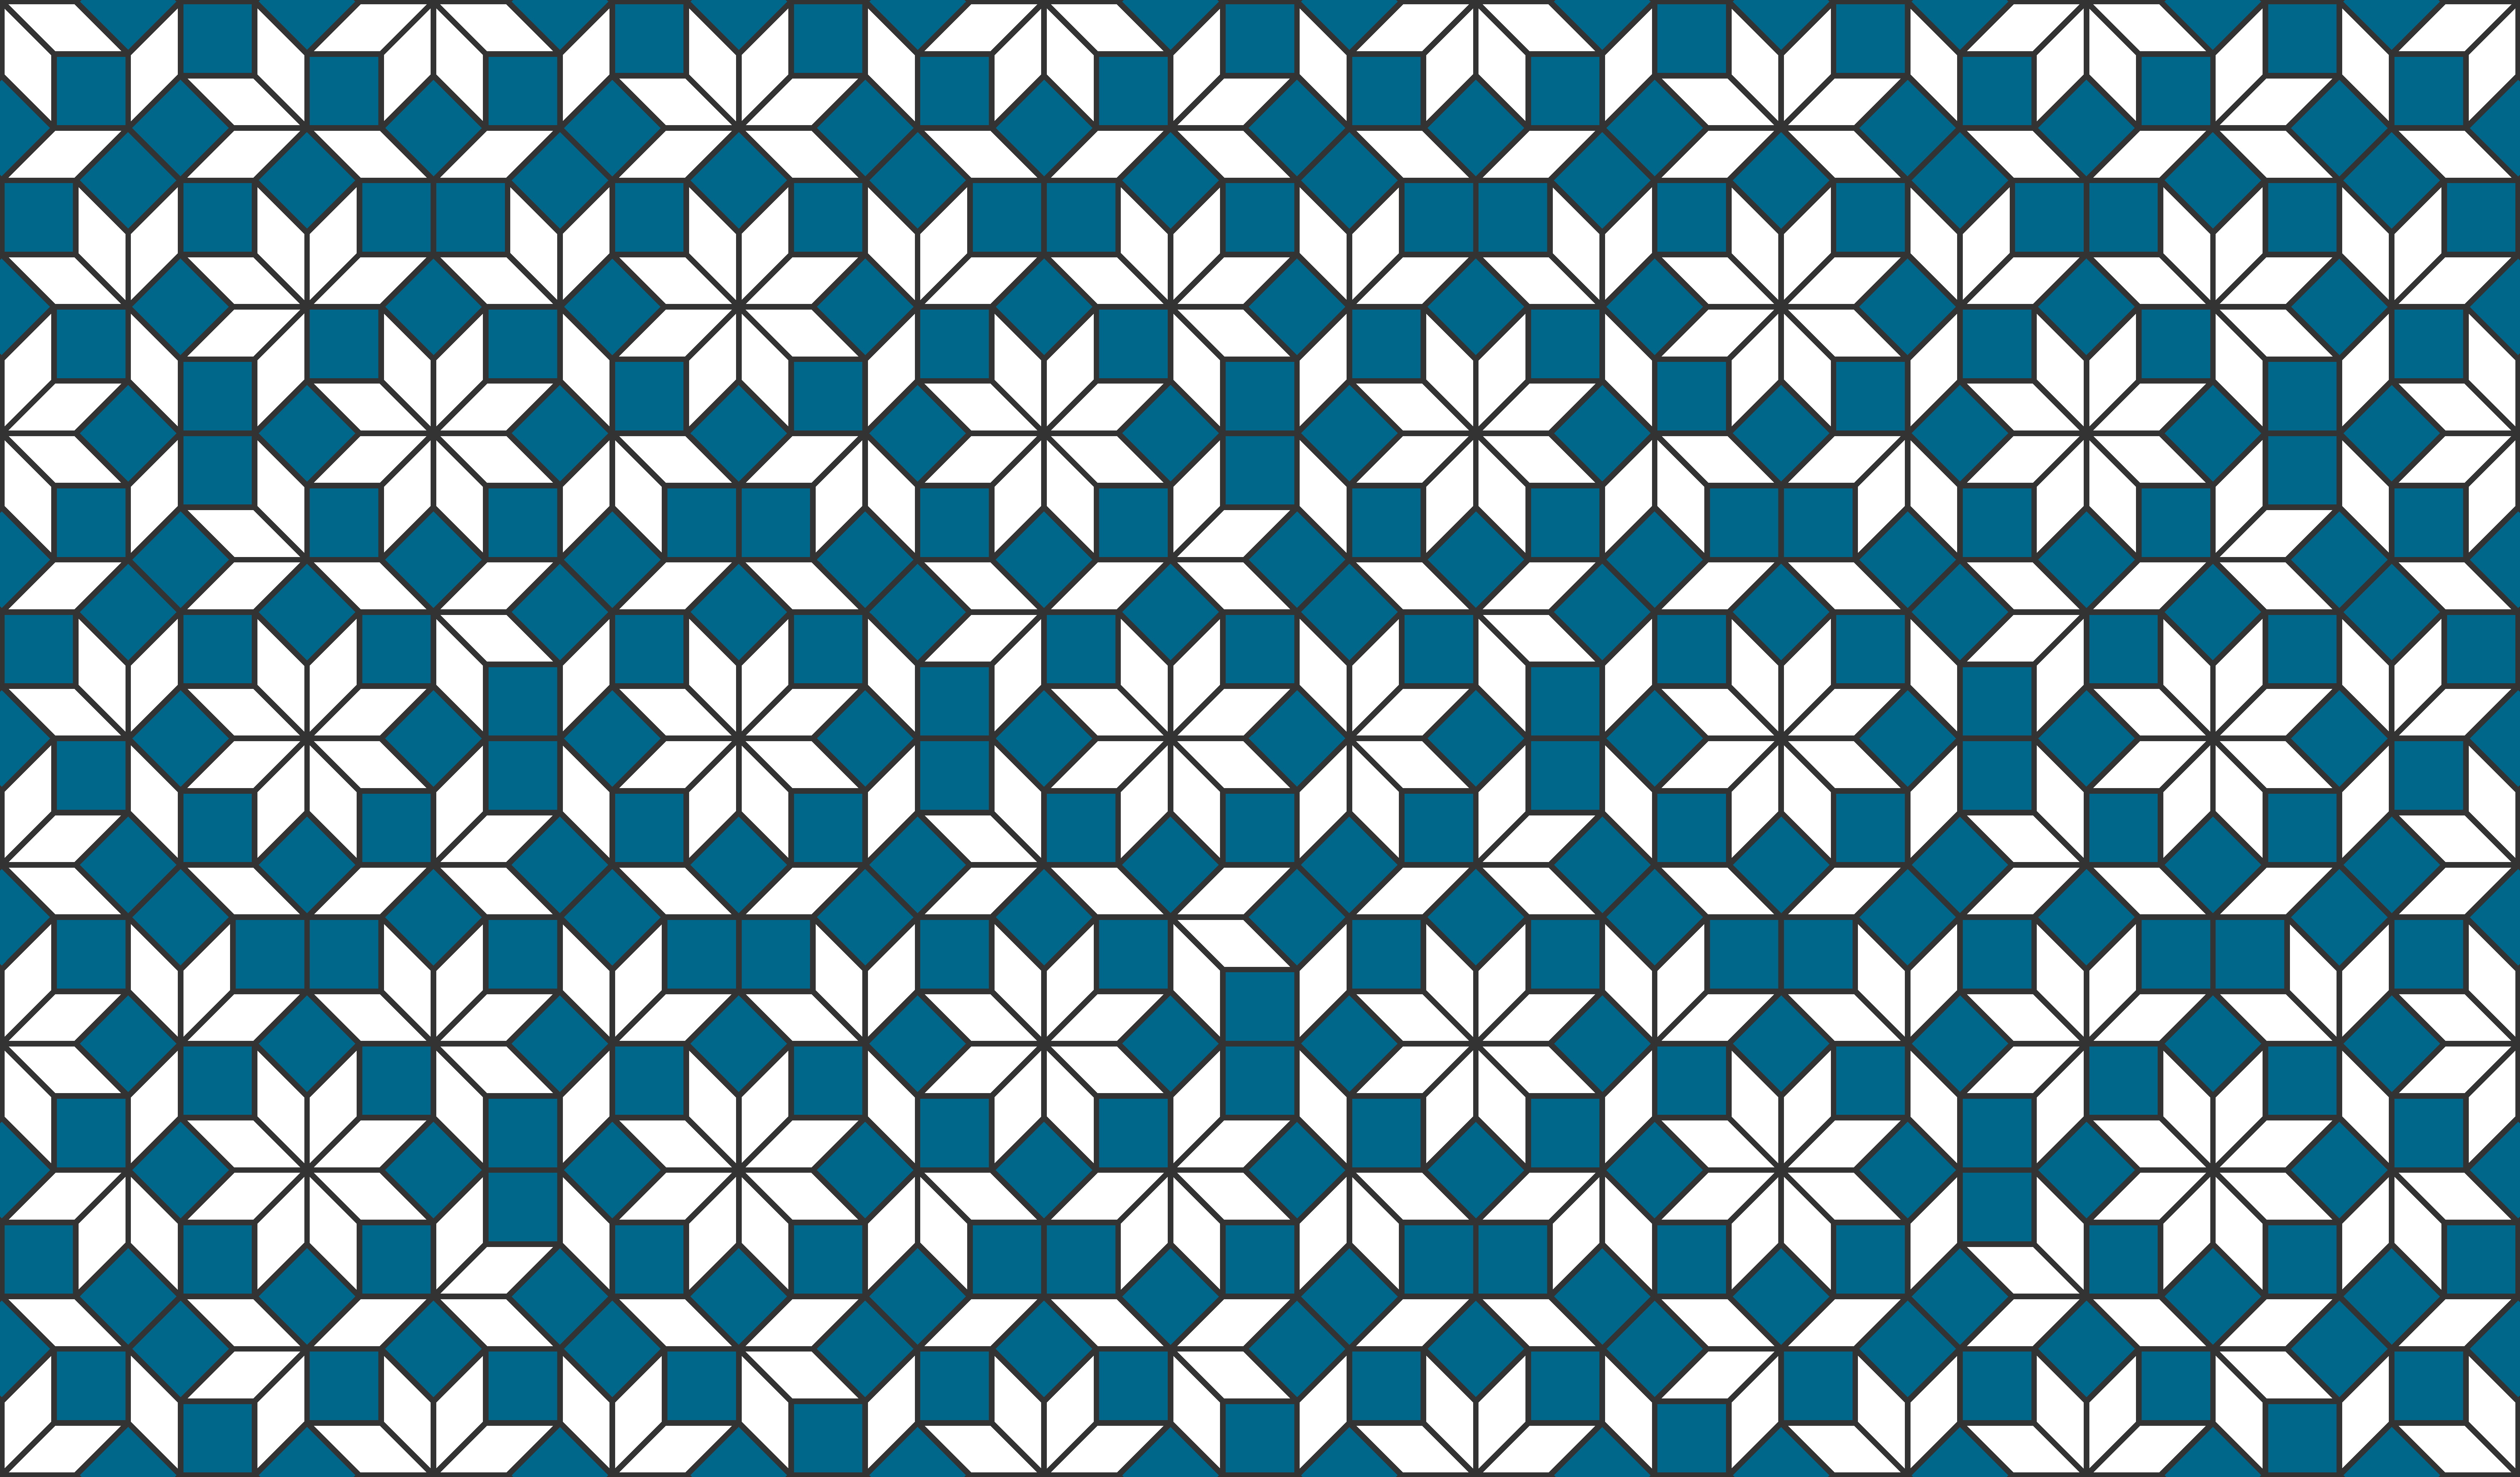
\includegraphics[width=1.\textwidth]{img/1_intro/ammann.pdf}

Patch of the Ammann-Beenker tiling.
\>
\)
\end{frame}

\begin{frame}{Periodic, quasiperiodic and random}
\only<1>{
A random tiling:

\centering
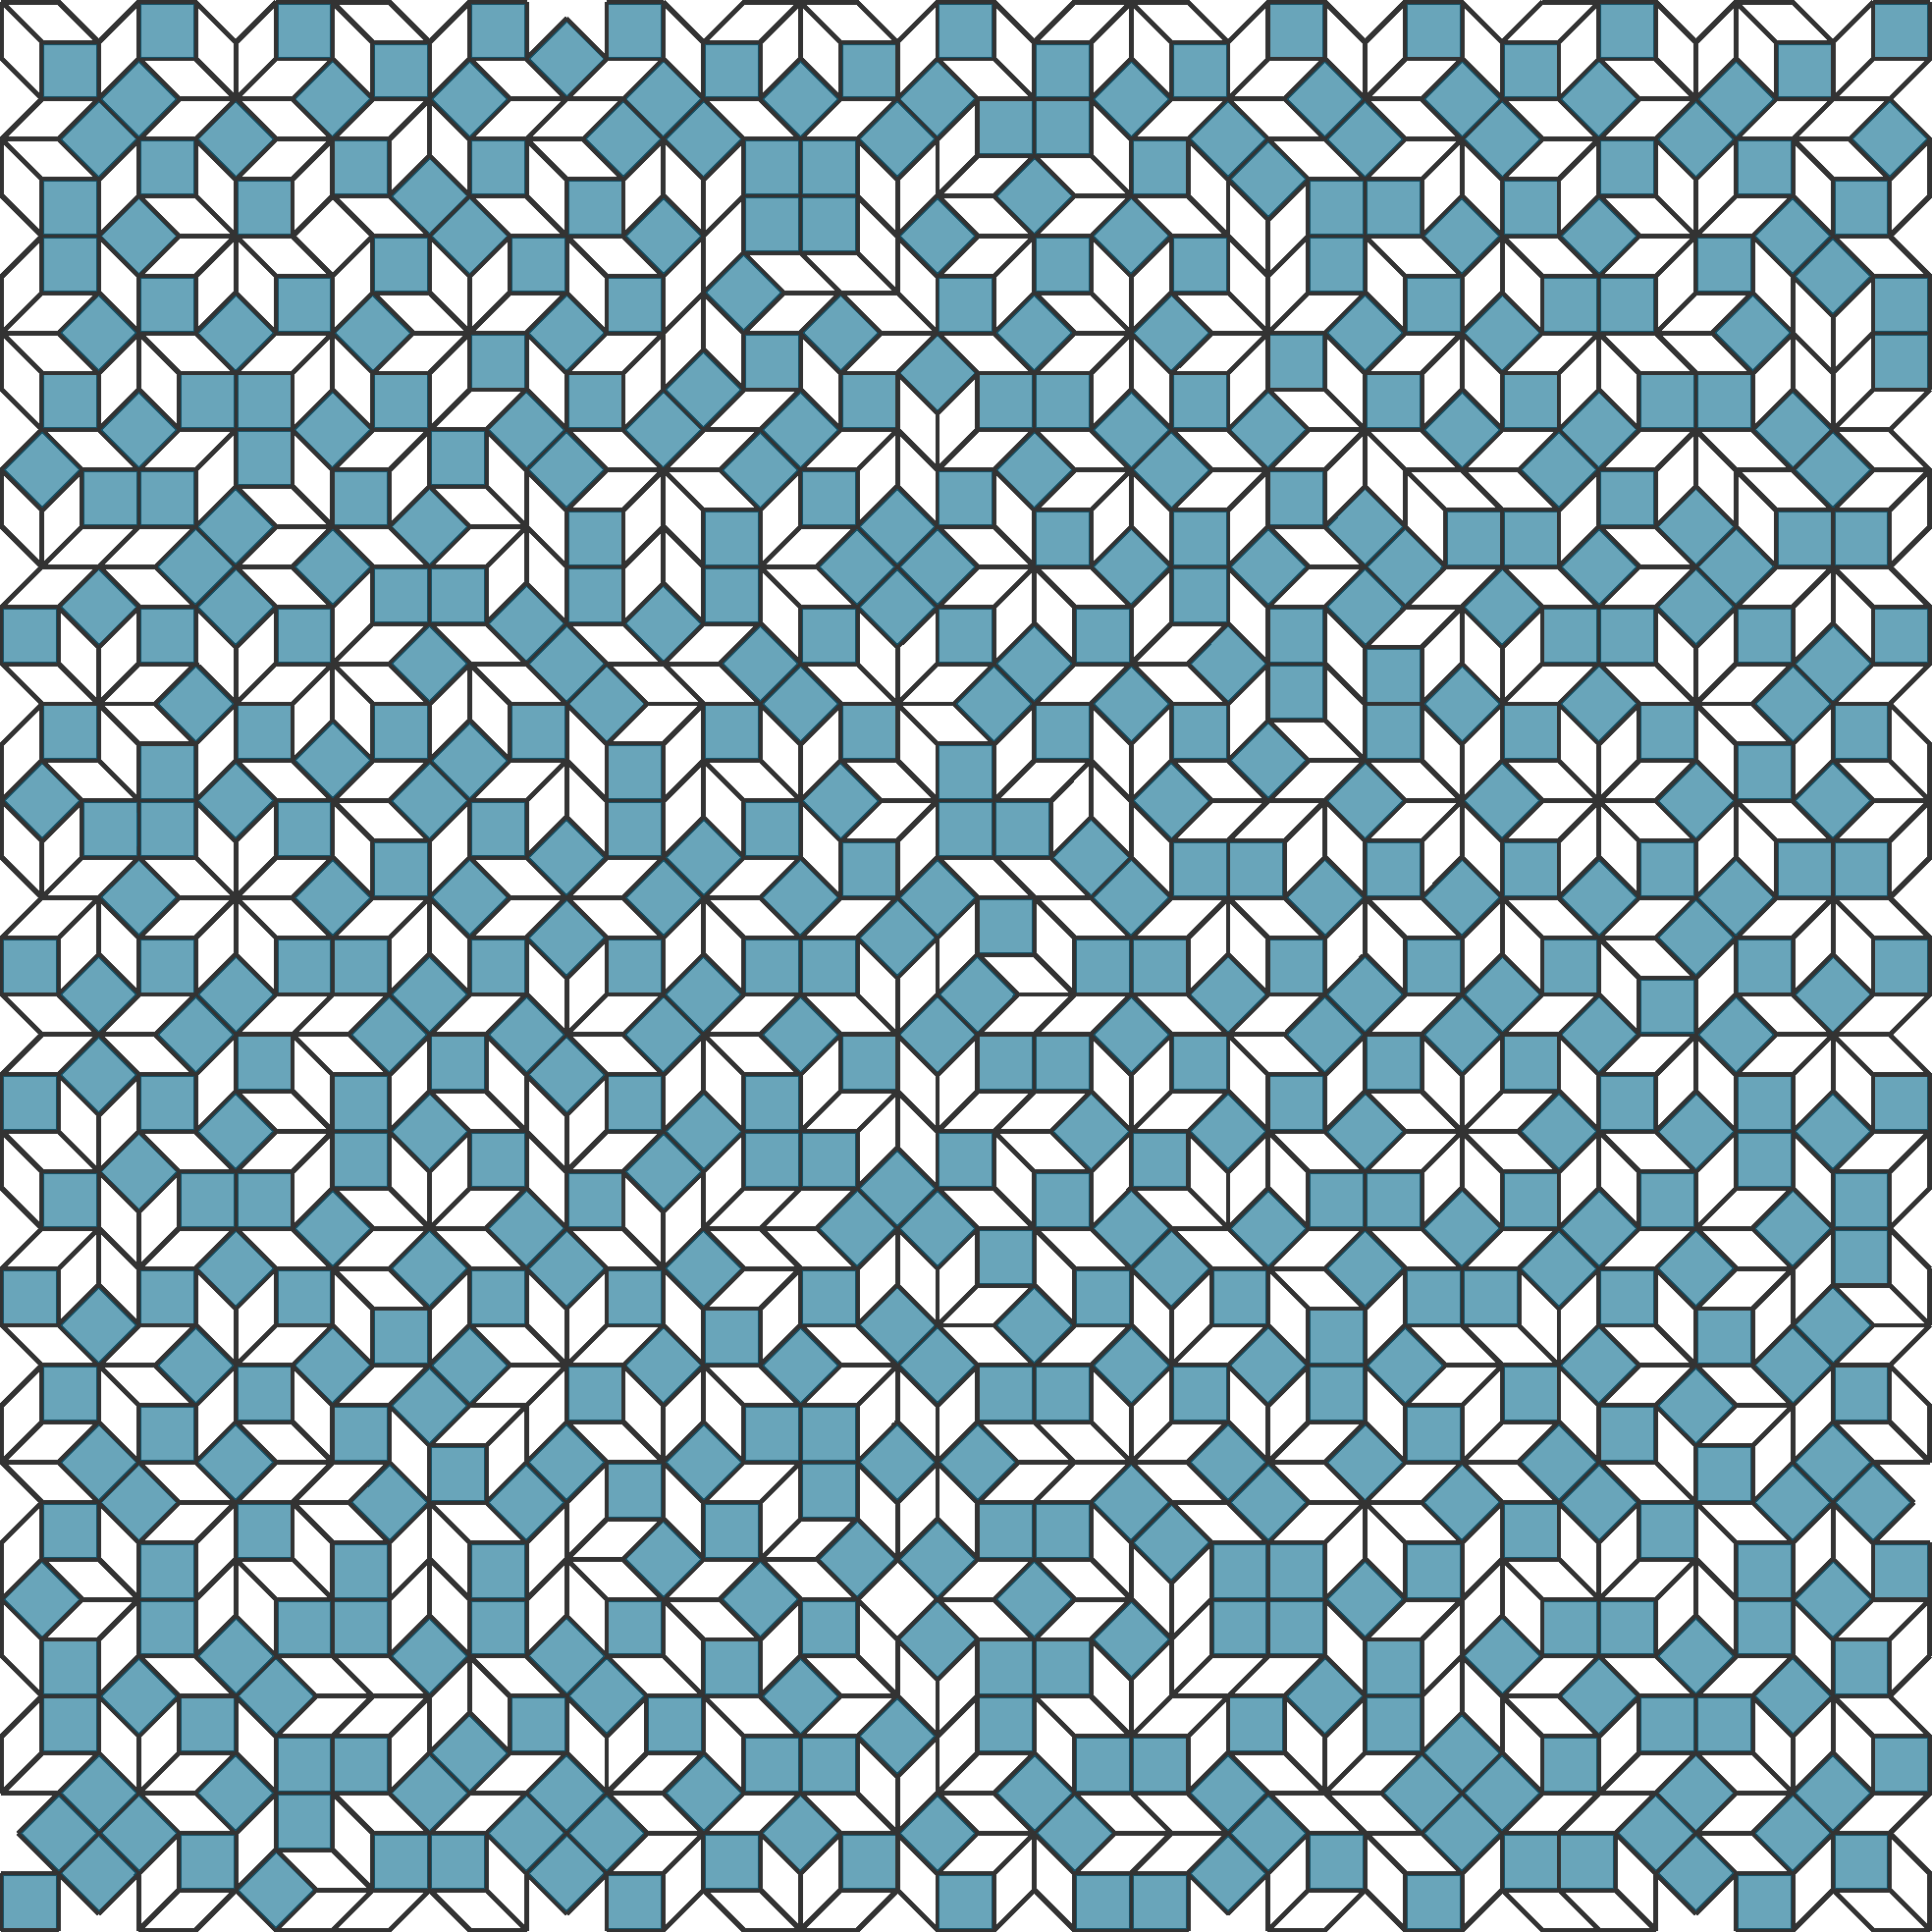
\includegraphics[width=.4\textwidth]{img/1_intro/random00.pdf}

}

\only<2>{
Two copies of the tiling:

\centering
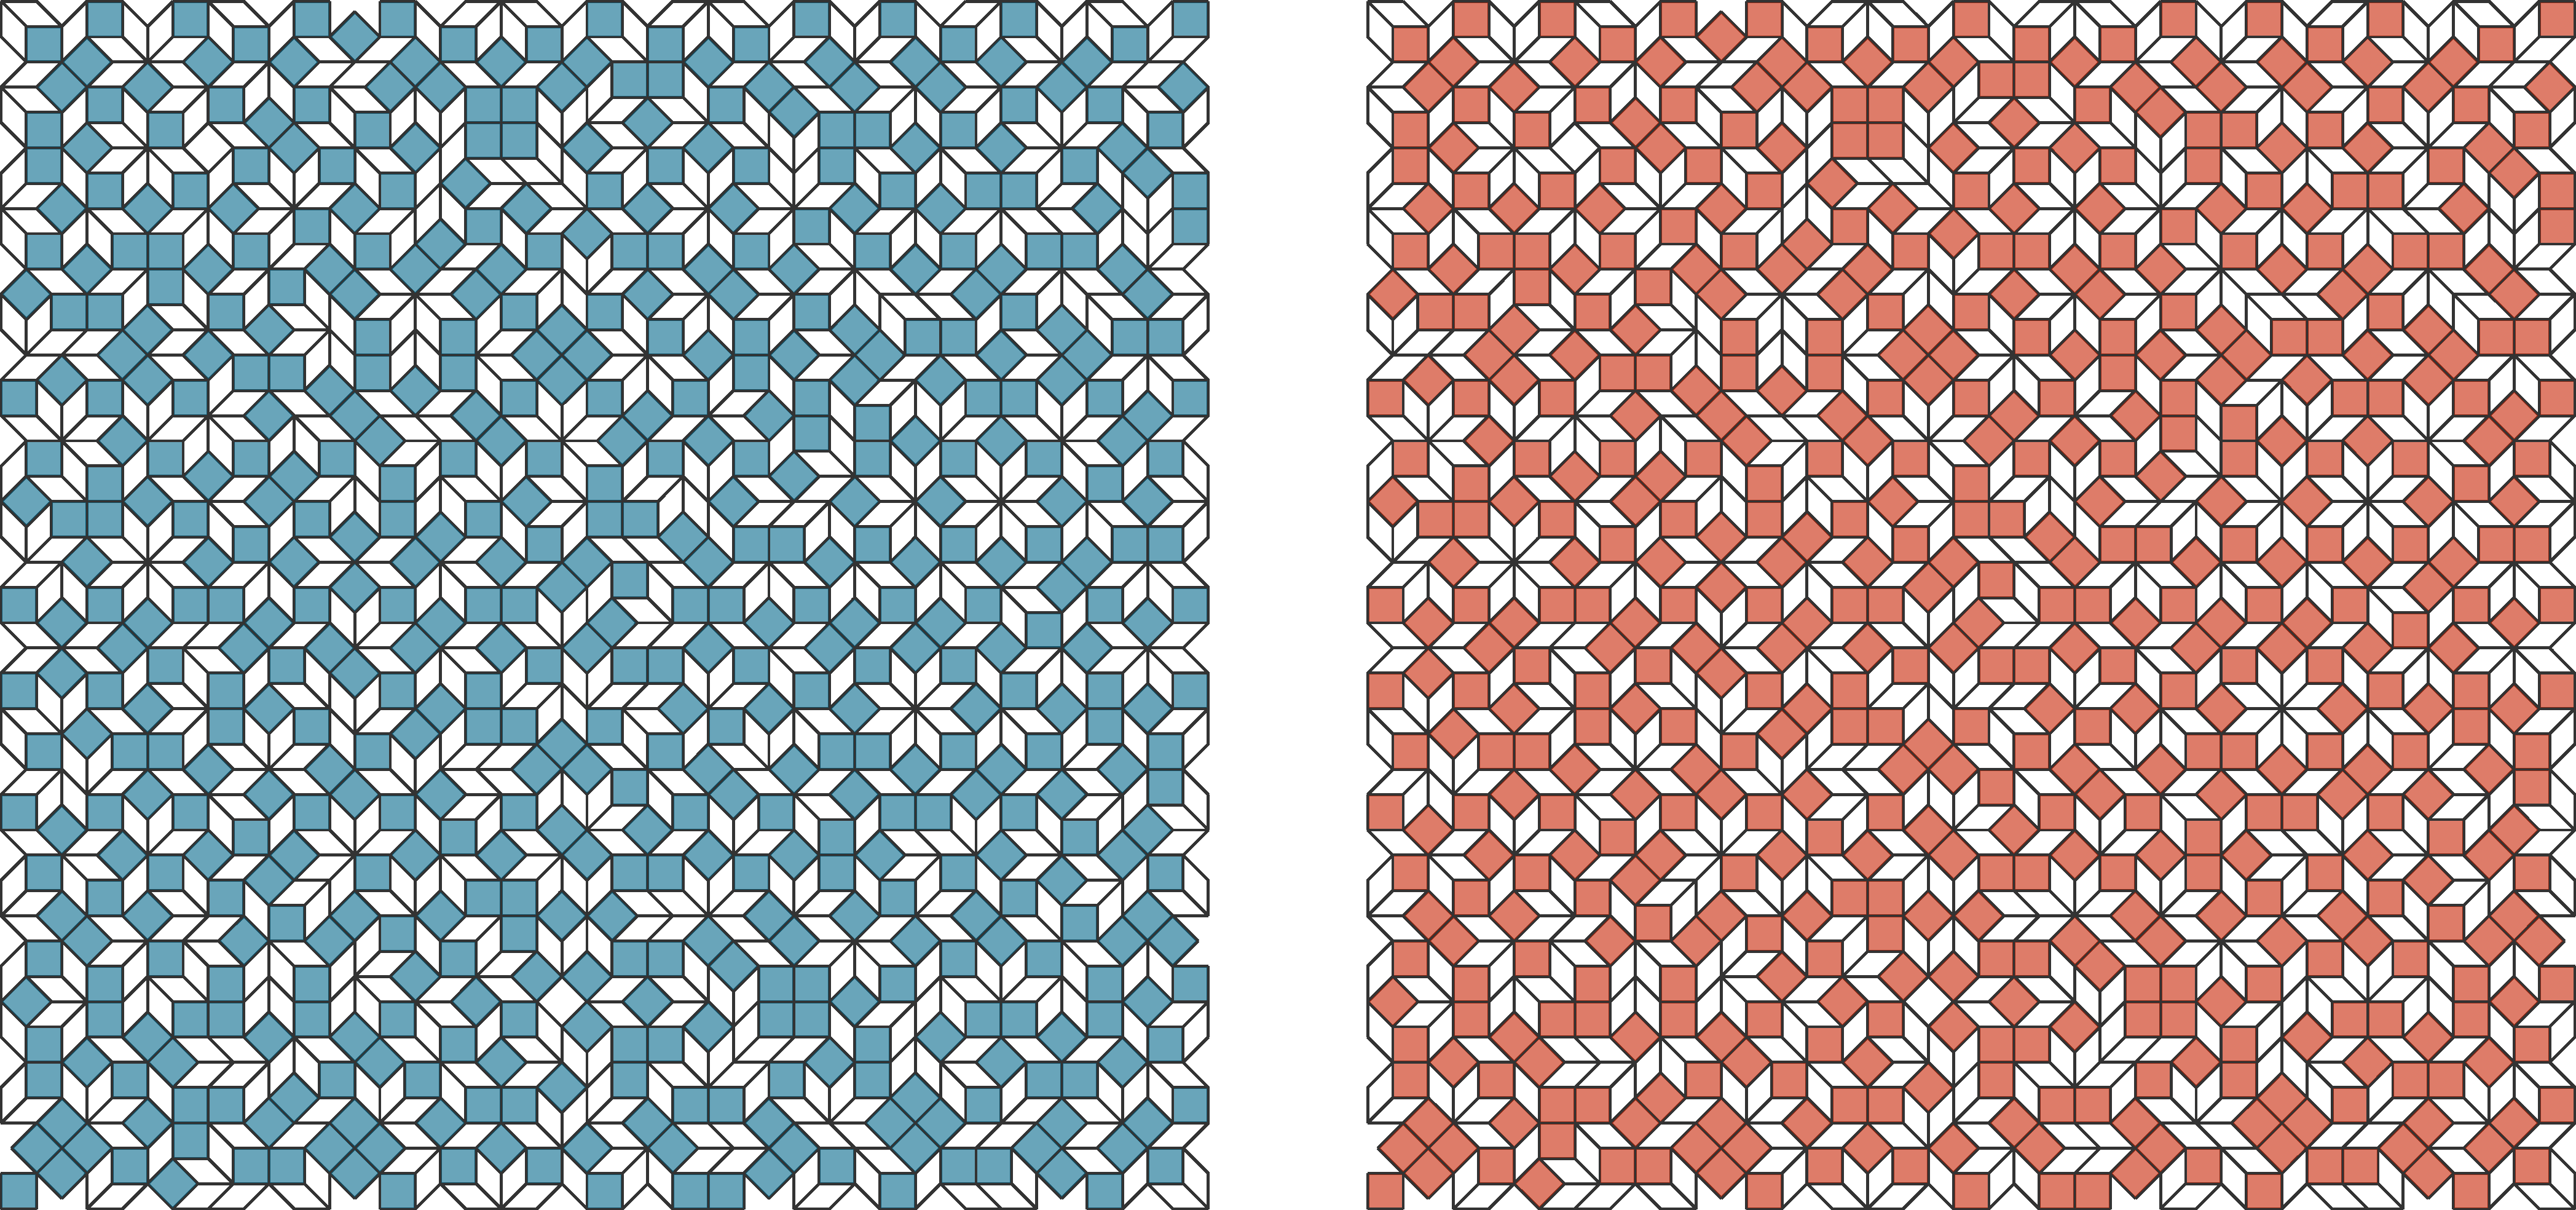
\includegraphics[width=.75\textwidth]{img/1_intro/random01.pdf}

}

\only<3>{
\centering
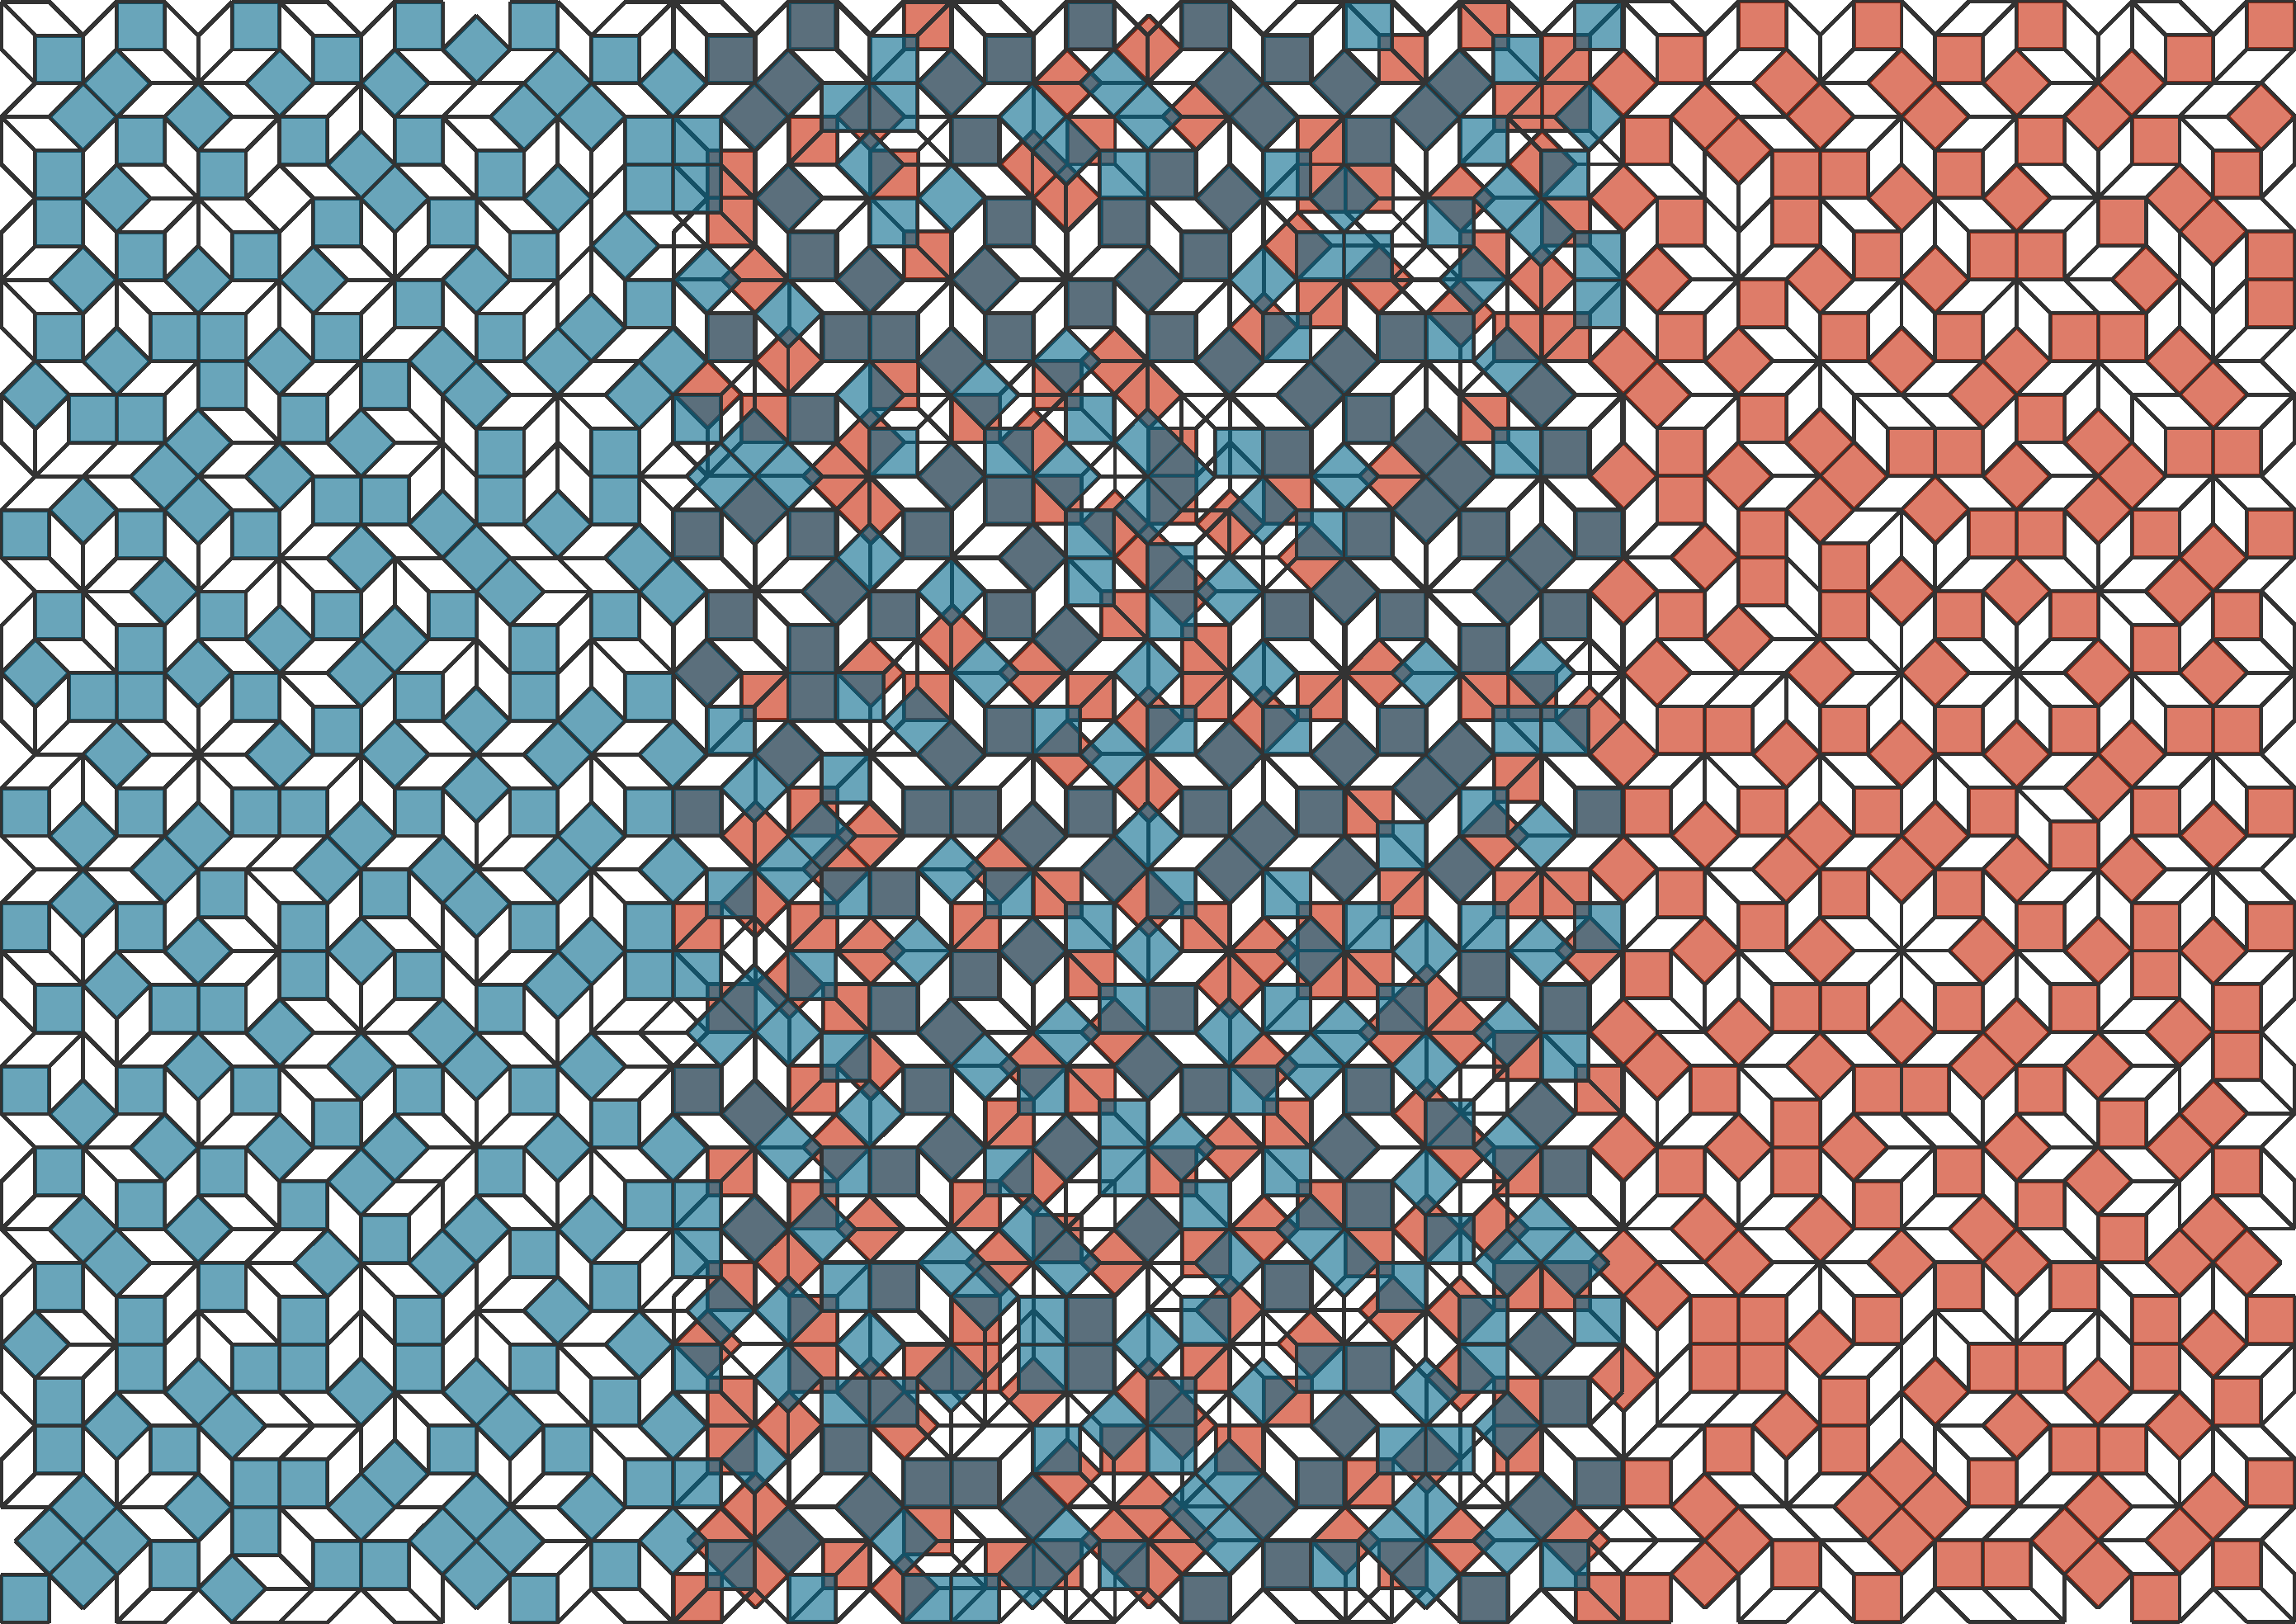
\includegraphics[width=.6\textwidth]{img/1_intro/random.pdf}

$\to$ no overlap $\to$ no order}

\centering
\only<4>{
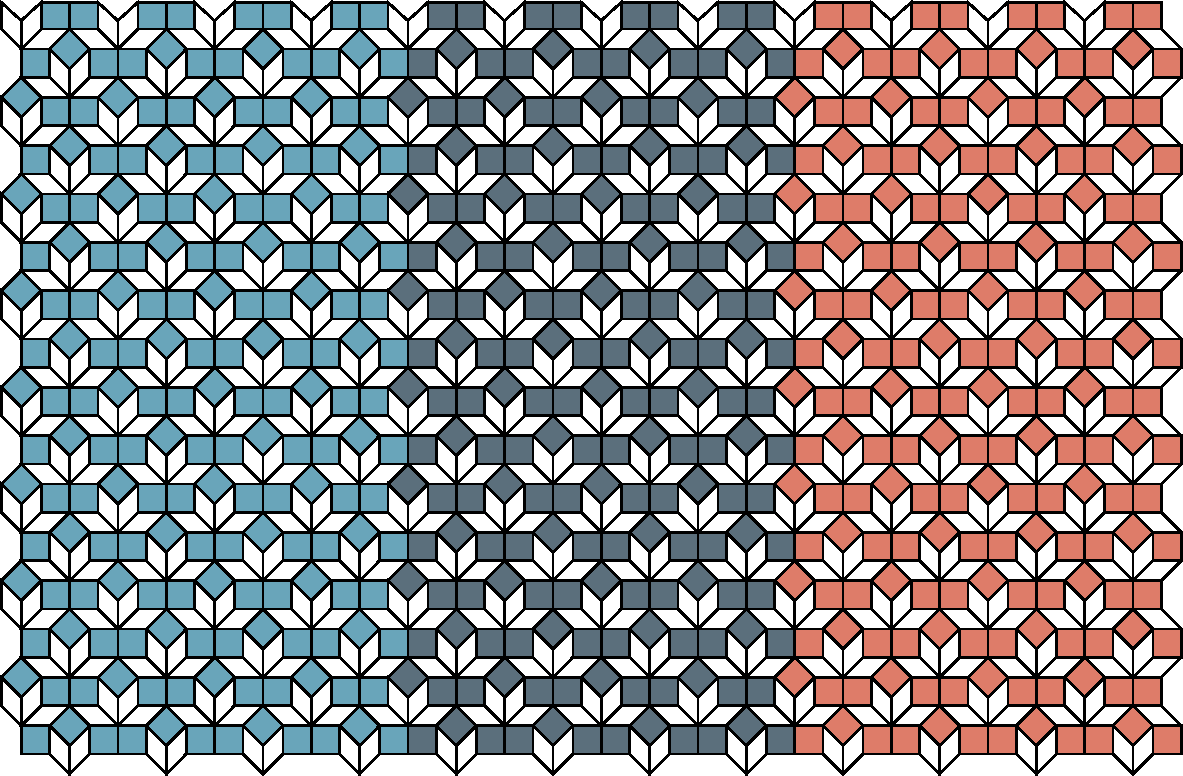
\includegraphics[width=.6\textwidth]{img/1_intro/periodic.pdf}

Perfect long range order: periodic}

\only<5>{
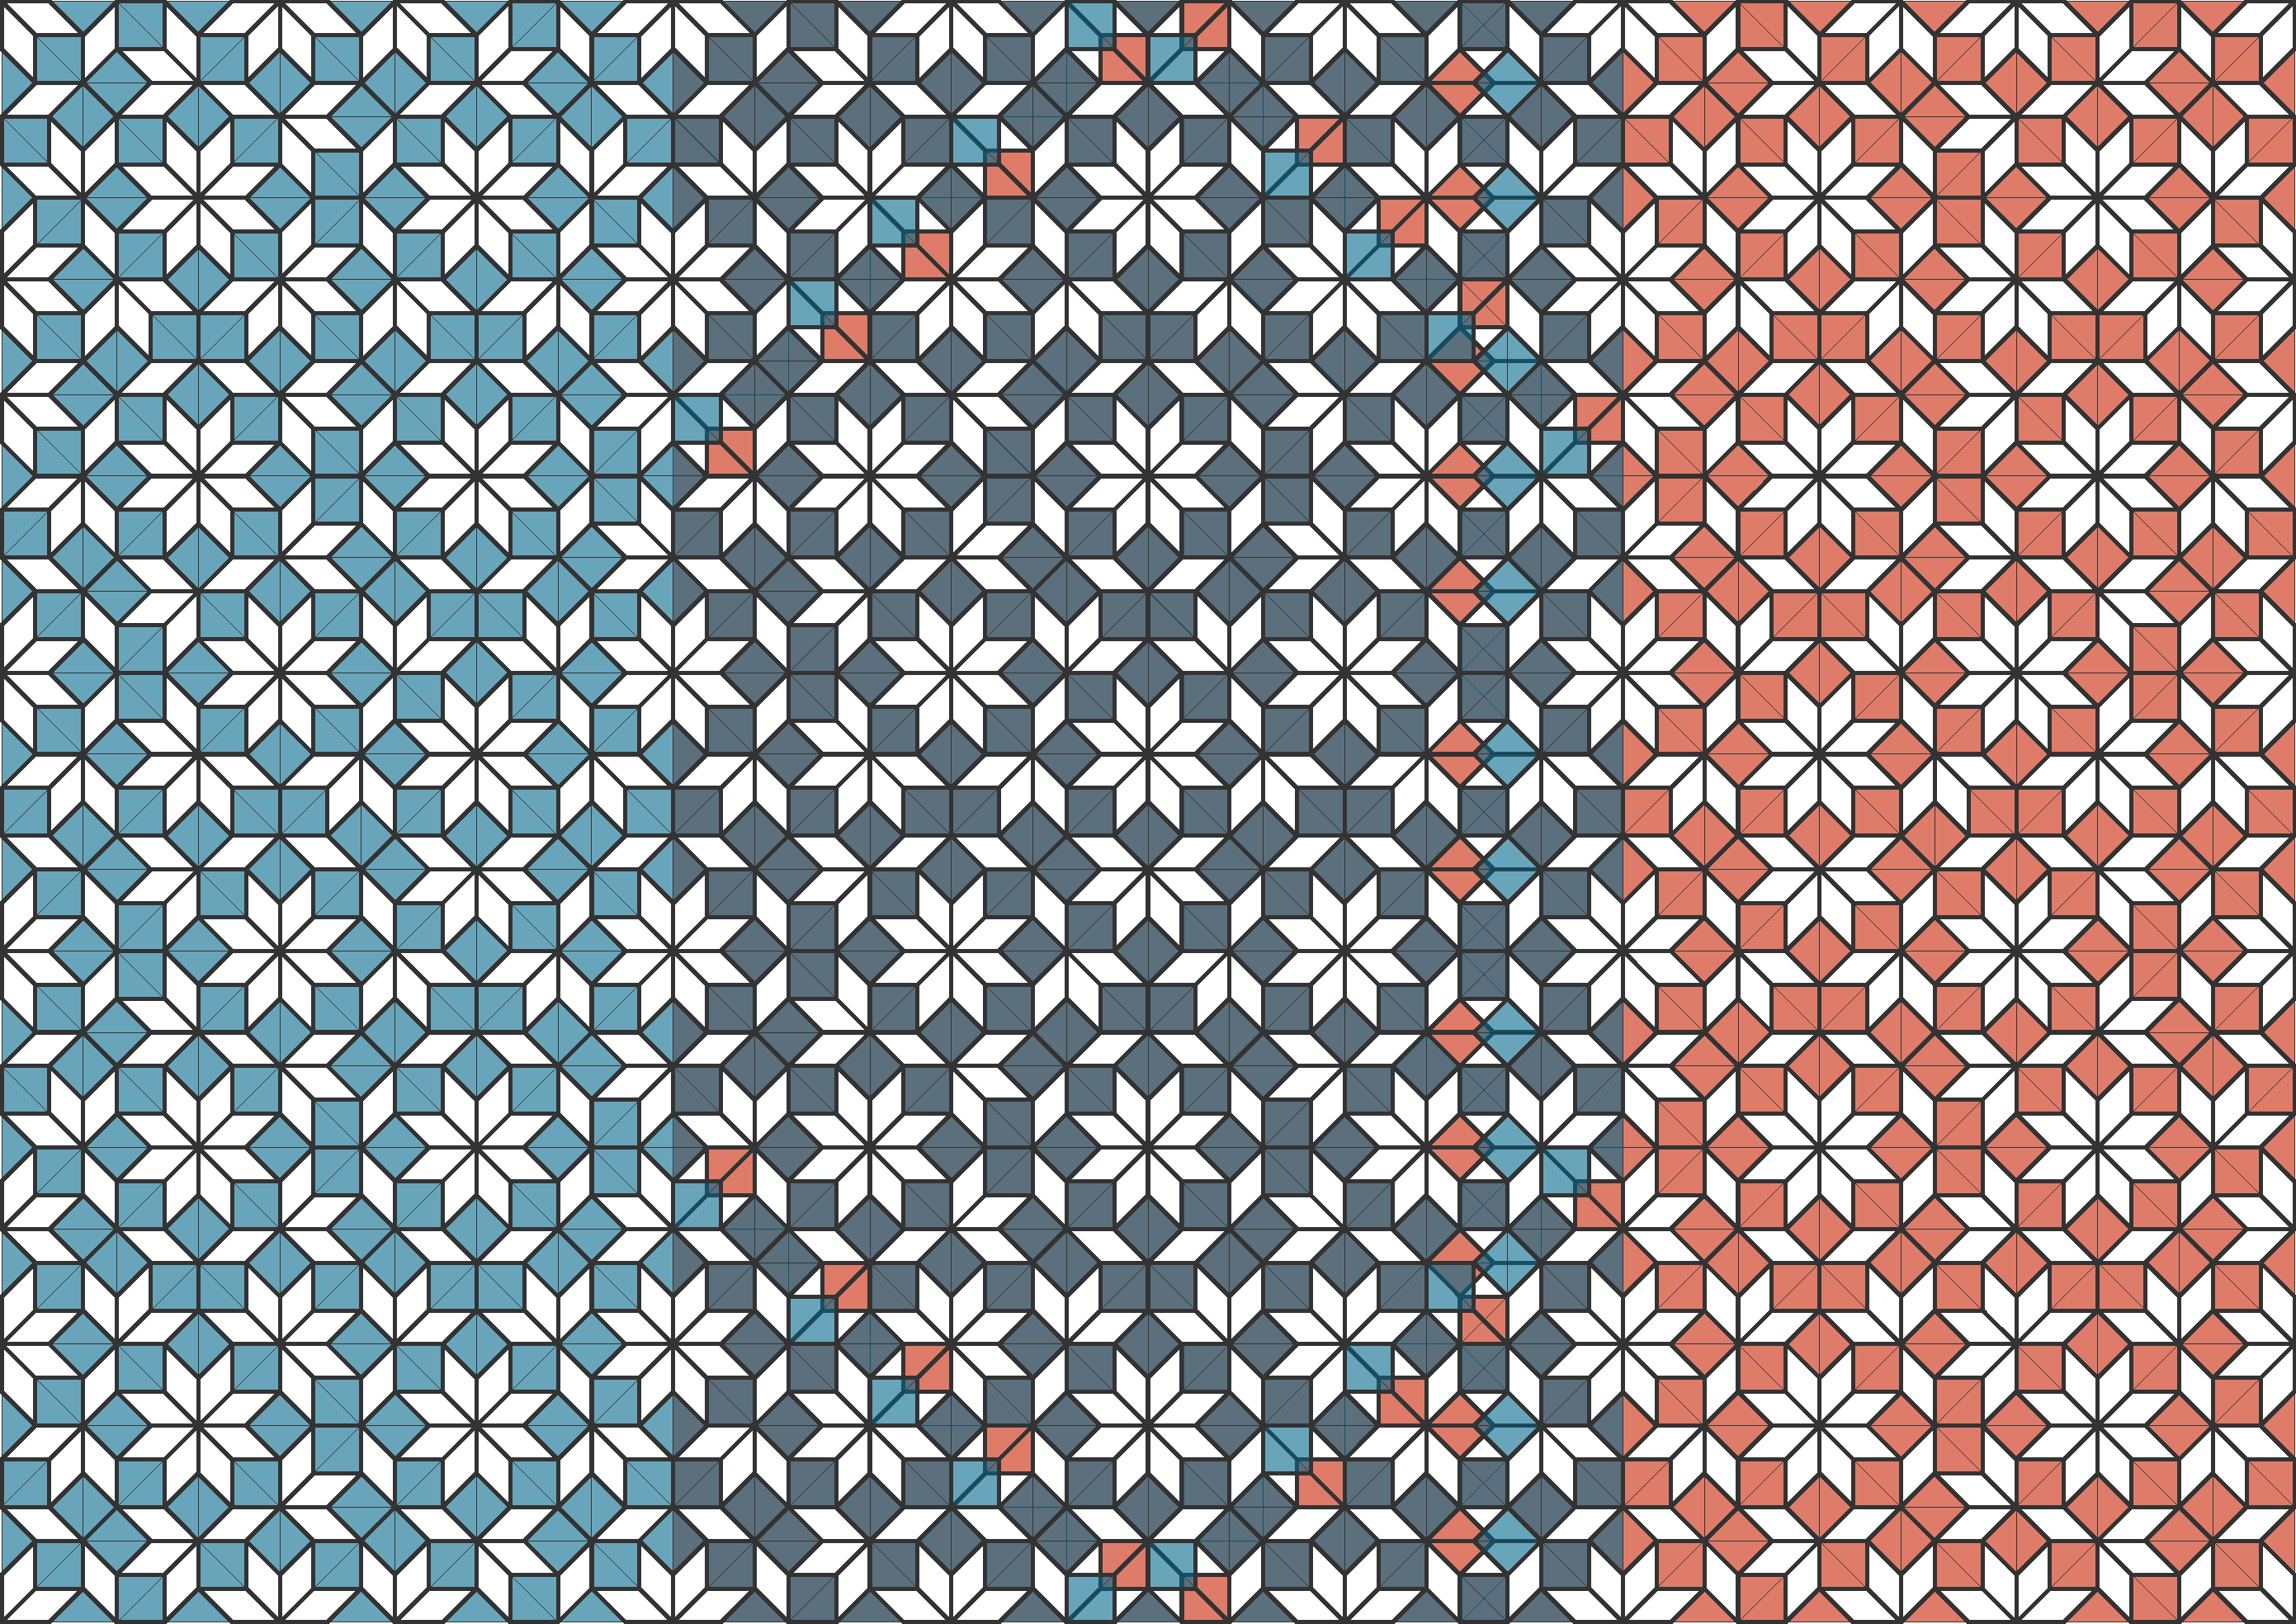
\includegraphics[width=.6\textwidth]{img/1_intro/quasiperiodic.pdf}

Long range order: quasiperiodic 

\flushleft{(see Chap.\ 2 of [Grimm, Baake 13])}
}

\end{frame}

%\begin{frame}{From tiles to atoms}
%Place atoms at the vertices of the tiling:
%
%{\centering
%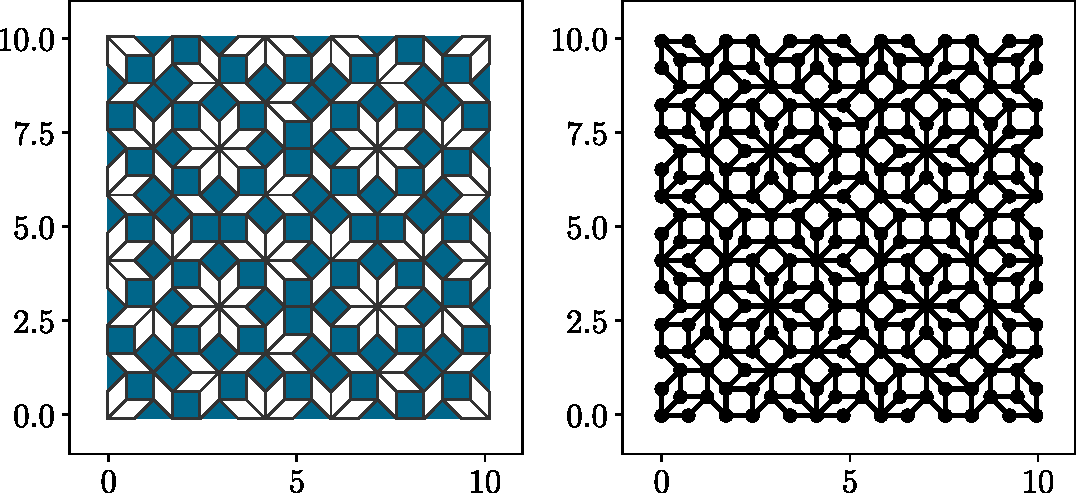
\includegraphics[width=.6\textwidth]{img/1_intro/AB_tiling_and_plot.pdf}
%
%}
%
%$\rightarrow$ can atoms arrange in such a quasiperiodic fashion?
%\end{frame}

\begin{frame}{Quasicrystals}
Quasicrystal $\to$ quasiperiodically arranged atoms:
\begin{itemize}
	\item \textbf{aperiodicity}
	\item \textbf{long range order} (diffraction pattern exhibits sharp peaks).
\end{itemize}
\(
	\<{6cm}
		\centering
		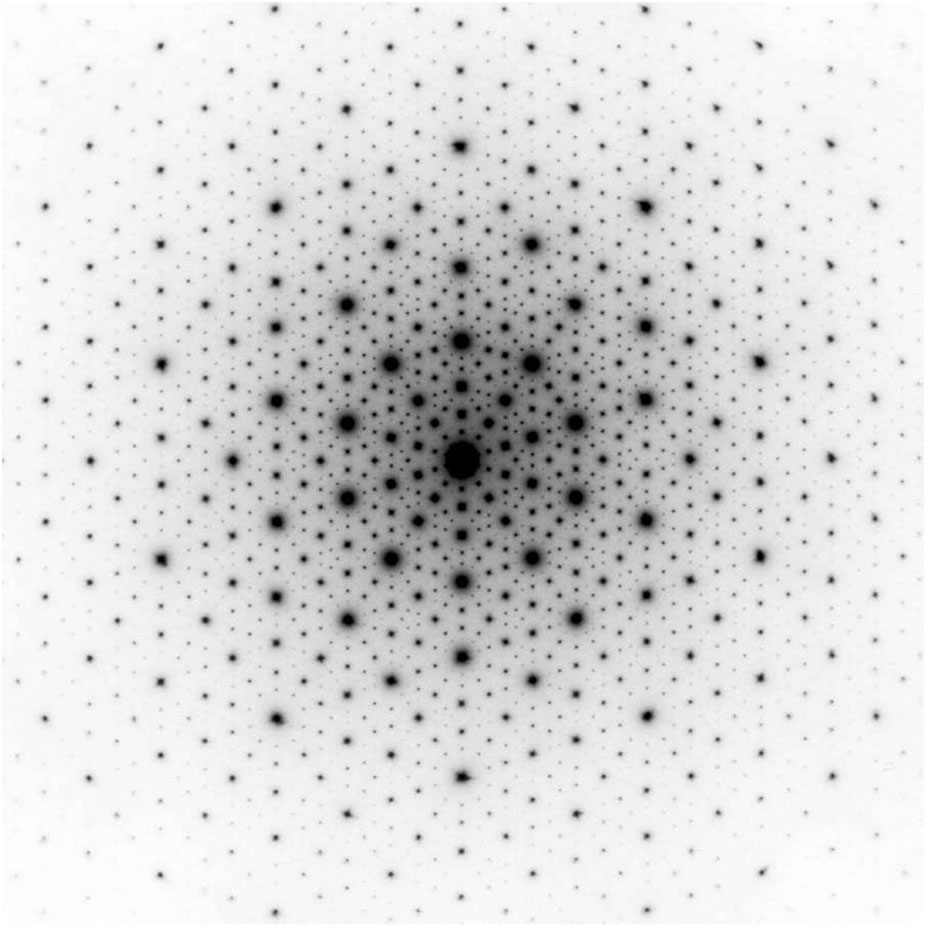
\includegraphics[scale=0.1]{img/1_intro/diffraction_tenfold.png}
		
		\ss{Diffraction pattern of a AlPdMn alloy} \ss{(Conradin Beeli group)}
	\>
	\<{6cm}
		\centering
		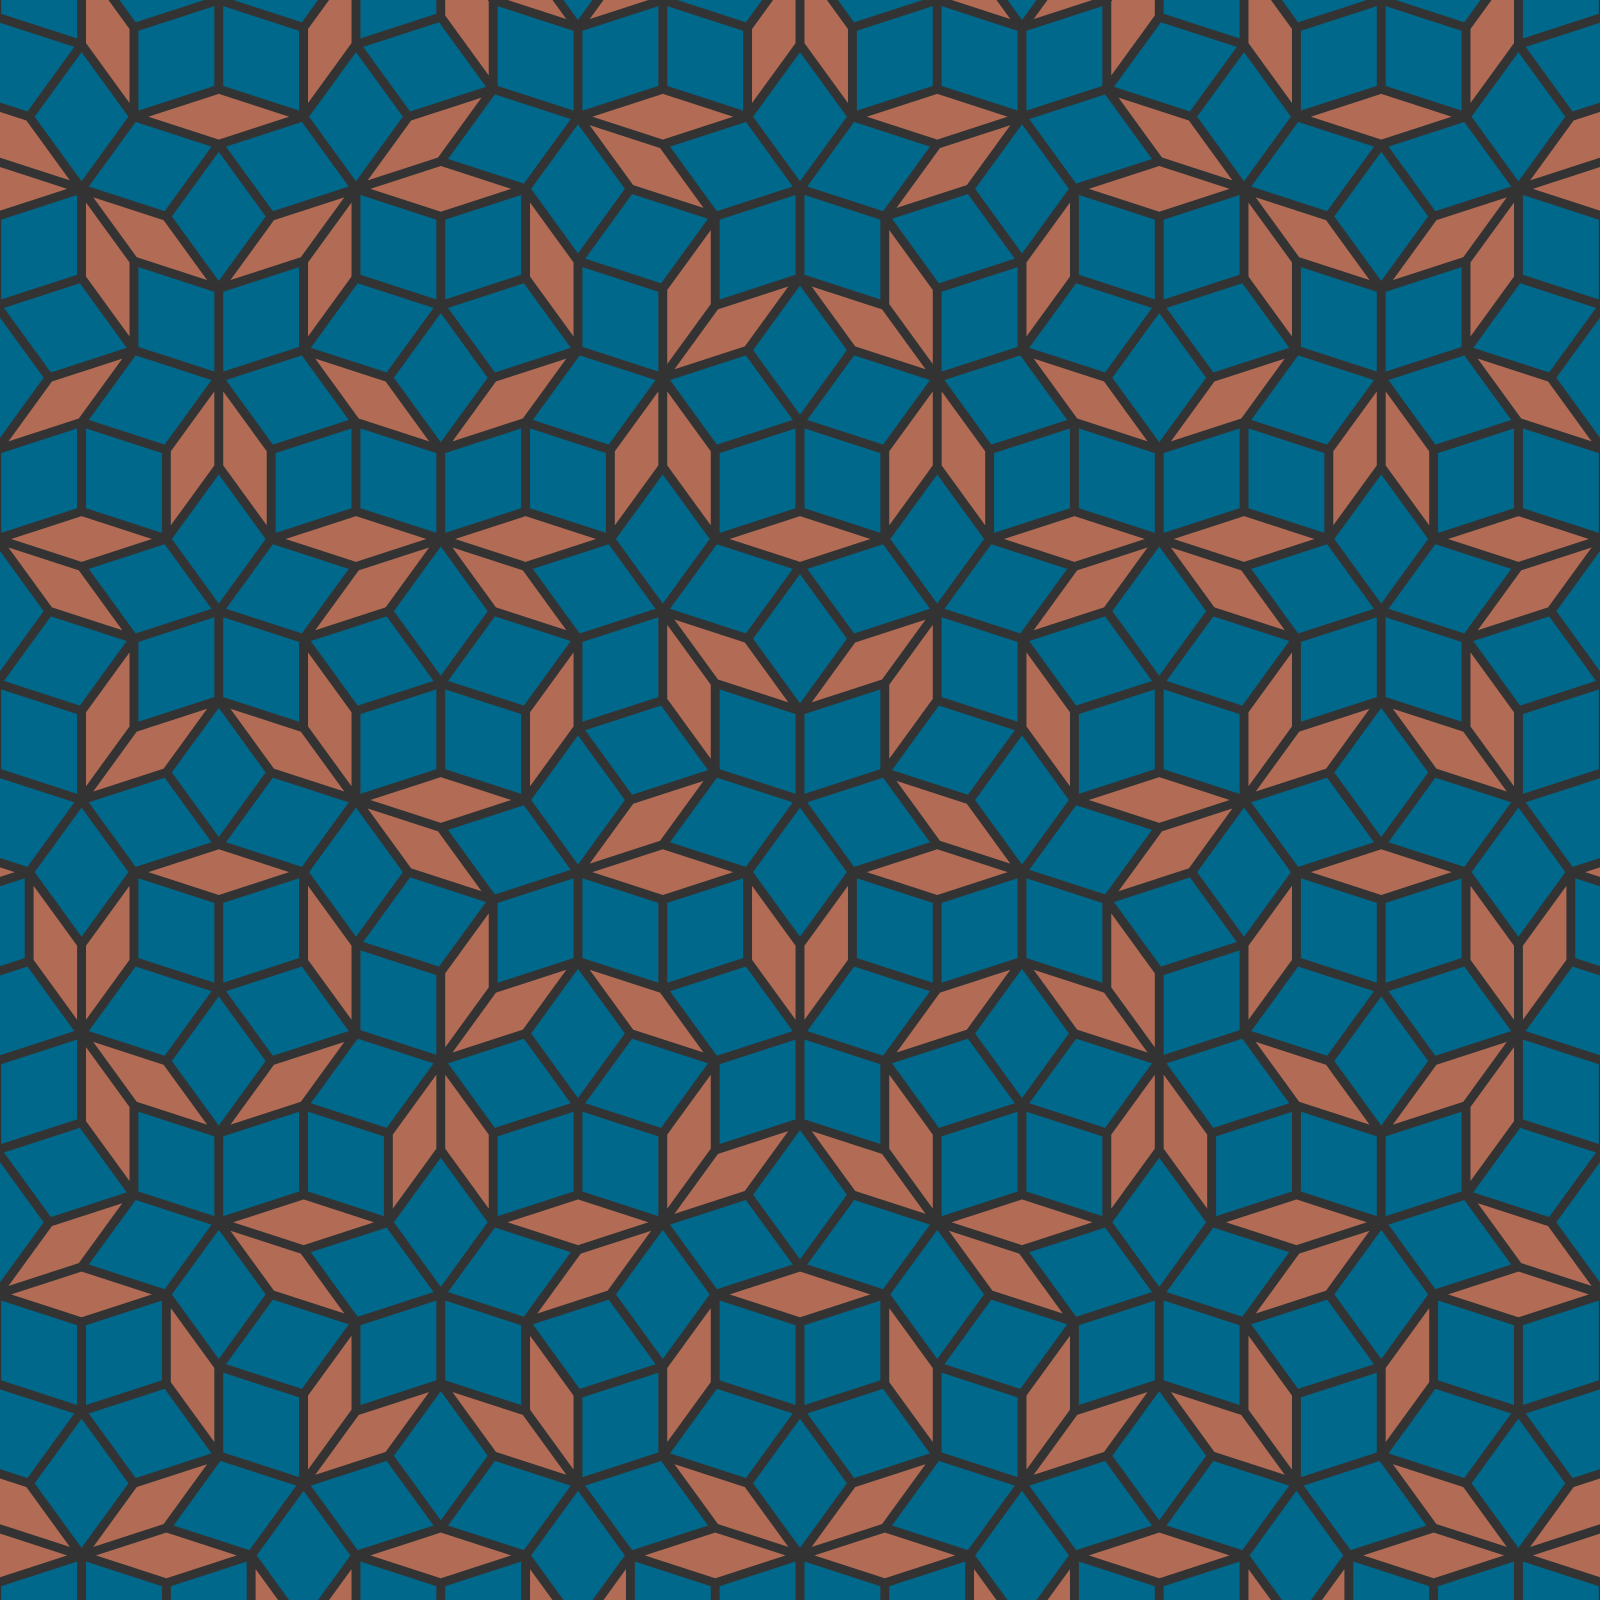
\includegraphics[scale=0.06]{img/1_intro/penrose.png}
		
		\ss{A patch of the quasiperiodic Penrose tiling,} \ss{used to model many quasicrystals.}
	\>
\)
\end{frame}

\begin{frame}{Artificial quasiperiodic structures}
\centering
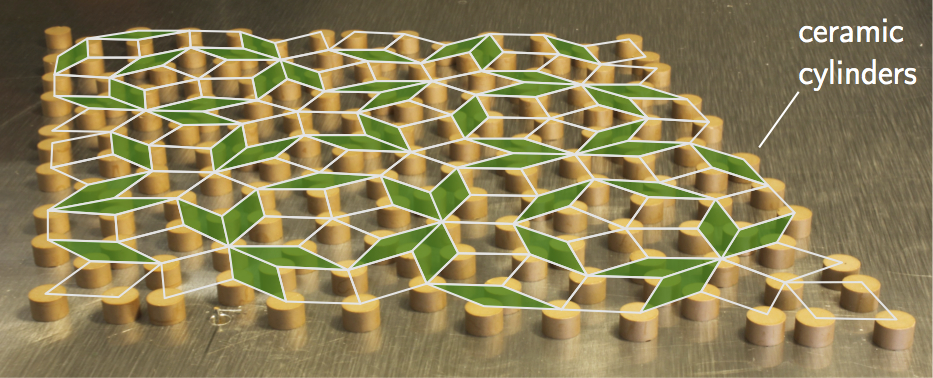
\includegraphics[width=.5\textwidth]{img/1_intro/dielectric_resonators.png}

{\ss{A network of dielectric resonators [Vignolo \etal{} 14]}}

\begin{itemize}
	\item Plasmons in semiconductor stacks [Merlin \etal{} 85]
	\item Microwaves in perforated metallic films [Matsui \etal{} 07]
	\item Microwaves in dielectric resonator networks [Vignolo \etal{} 14]
	\item Light solitons [Freedman \etal{} 07]
	\item Cold atoms in laser potentials [Guidoni \etal{} 97]
	\item Polaritons in wire cavities [Tanese \etal{} 14]
\end{itemize}
\end{frame}


\begin{frame}{Fractals}
Fractal: object invariant under rescaling
\(
\<{7cm}
\centering
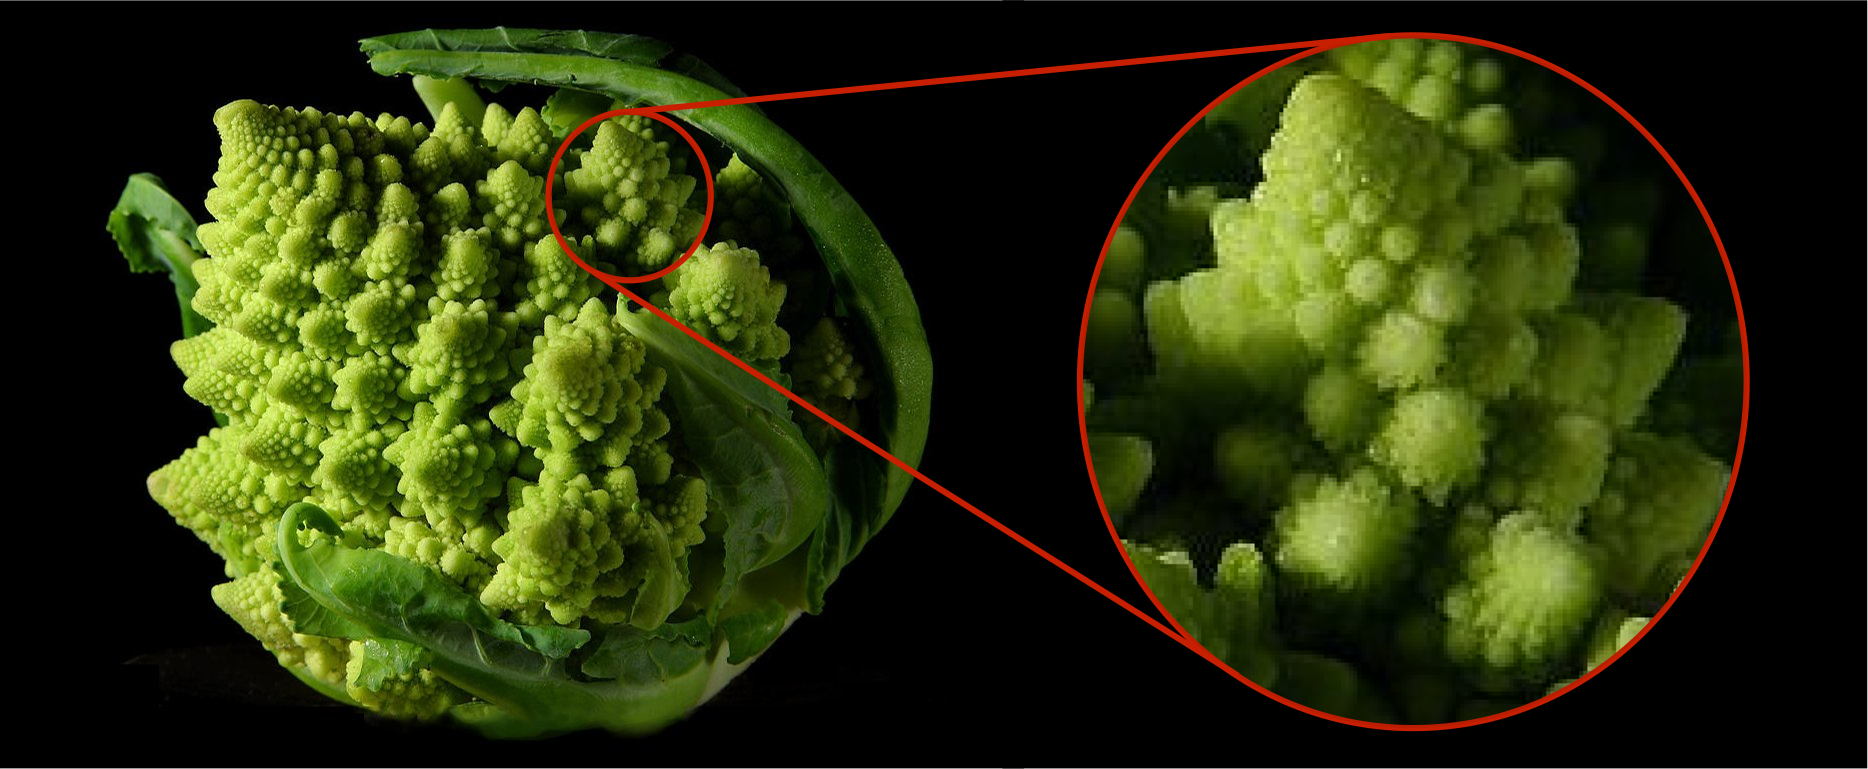
\includegraphics[width=1.\textwidth]{img/1_intro/Fractal_Broccoli.png}

{\ss Romanesco broccoli (\copyleft{} Wikimedia commons)}
\>
\<{7cm}
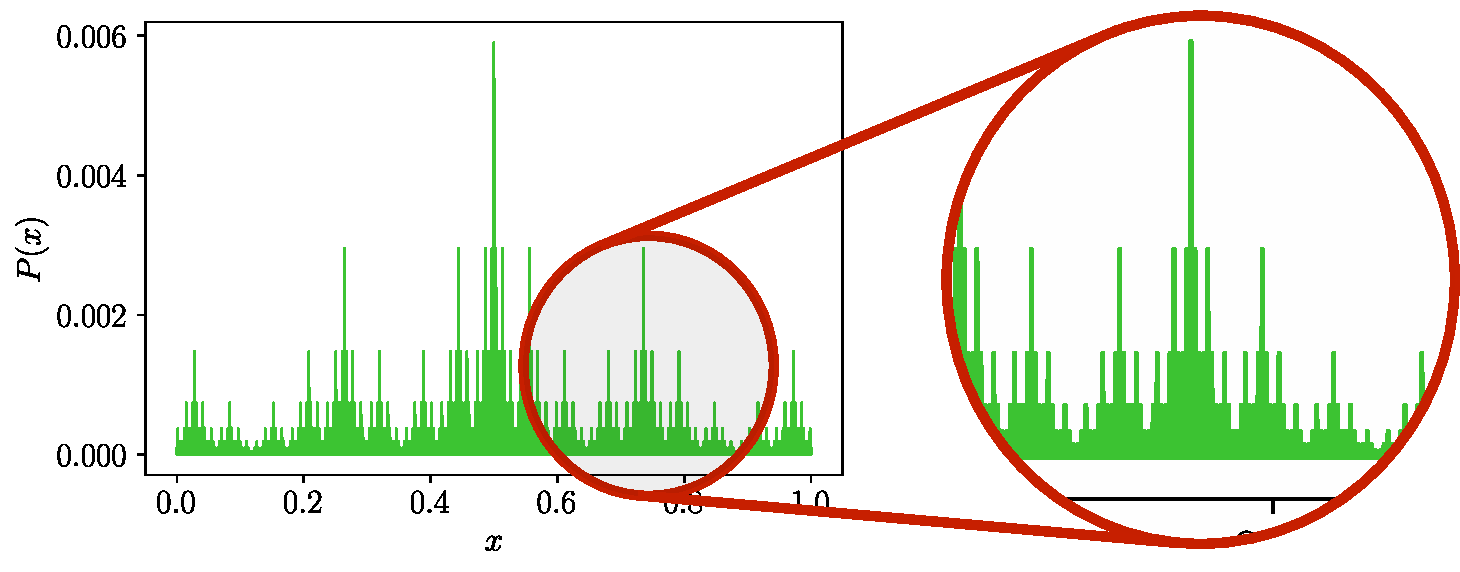
\includegraphics[width=1.\textwidth]{img/1_intro/heights.pdf}

{\ss Electronic density along a quasiperiodic chain}
\>
\)

Quasicrystals \emph{not} fractal\dots

\dots but electrons on quasicrystals $\to$ fractal behavior

\begin{beamerboxesrounded}%
        [shadow=true]%
        {Goal:}
\textbf{Link the fractal behavior of the electrons to quasiperiodicity}
\end{beamerboxesrounded}
\end{frame}

\begin{frame}{Fractal dimensions}
\begin{itemize}
	\item $M(L) \propto L^d$ for a non-fractal $d$-dimensional object\dots What happens for a fractal one?
	
	{\centering
	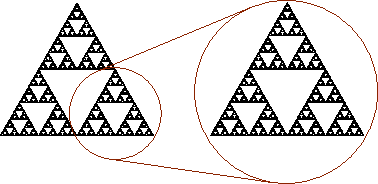
\includegraphics[width=.4\textwidth]{img/2_part1/sierpinski}
	
	{\ss A Sierpiński triangle}
	
	}
	
	\[
		M(L) \sim L^{d_0} \text{, with } d_0 = \log 3/\log 2
	\]
	
	\item $d_0$ is the Hausdorff fractal dimension
	\item $1 < d_0 \simeq 1.58 < 2$, signature of a fractal object
	\item Probe fractality of the $q^\text{th}$ moment of a distribution $\to$ generalized fractal dimensions $d_q$.
\end{itemize}
\end{frame}